% !TeX root = ./main.tex
\documentclass{article}

\usepackage[utf8]{inputenc}
\usepackage{graphicx}
\usepackage{amsmath}
\usepackage[english]{babel}
\usepackage[pdfborderstyle={/S/U/W 0}, colorlinks=true,allcolors=blue]{hyperref}
\urlstyle{same}

\begin{document}

\title{Linear classification of the IRIS dataset}
\author{Leik Lima-Eriksen og Torbjørn Bratvold}
\date{April 2020}

\maketitle

\section{Introduction}
The project described in this report has the goal of classifying samples of Iris flowers into
three different classes, namely the Setosa, Versicolor, and the Virginica. Classifying plants
based on their dimensions has multiple usages. For instance, it may be used by botanics as a tool
for easing their job. Also, it could be useful for mushroom enthusiasts to detect poisonous
mushrooms. And since classification algorithms may detect connections between classes and features
which may be hard for even the trained eye to spot, it could potentially outperform humans and
avoid disastrous misclassifications.

The Iris flowers have large (Sepal) and small (Petal) leaves, and the length and width of these
varies according to the class of flower. Thus, it seems natural to use these dimensions as features
for the classification. A dataset consisting of such measurements has been used in this project. 50
samples from each class has been provided. Their distributions are summarized in \autoref{fig:histograms}.

\begin{figure}
    \centering
    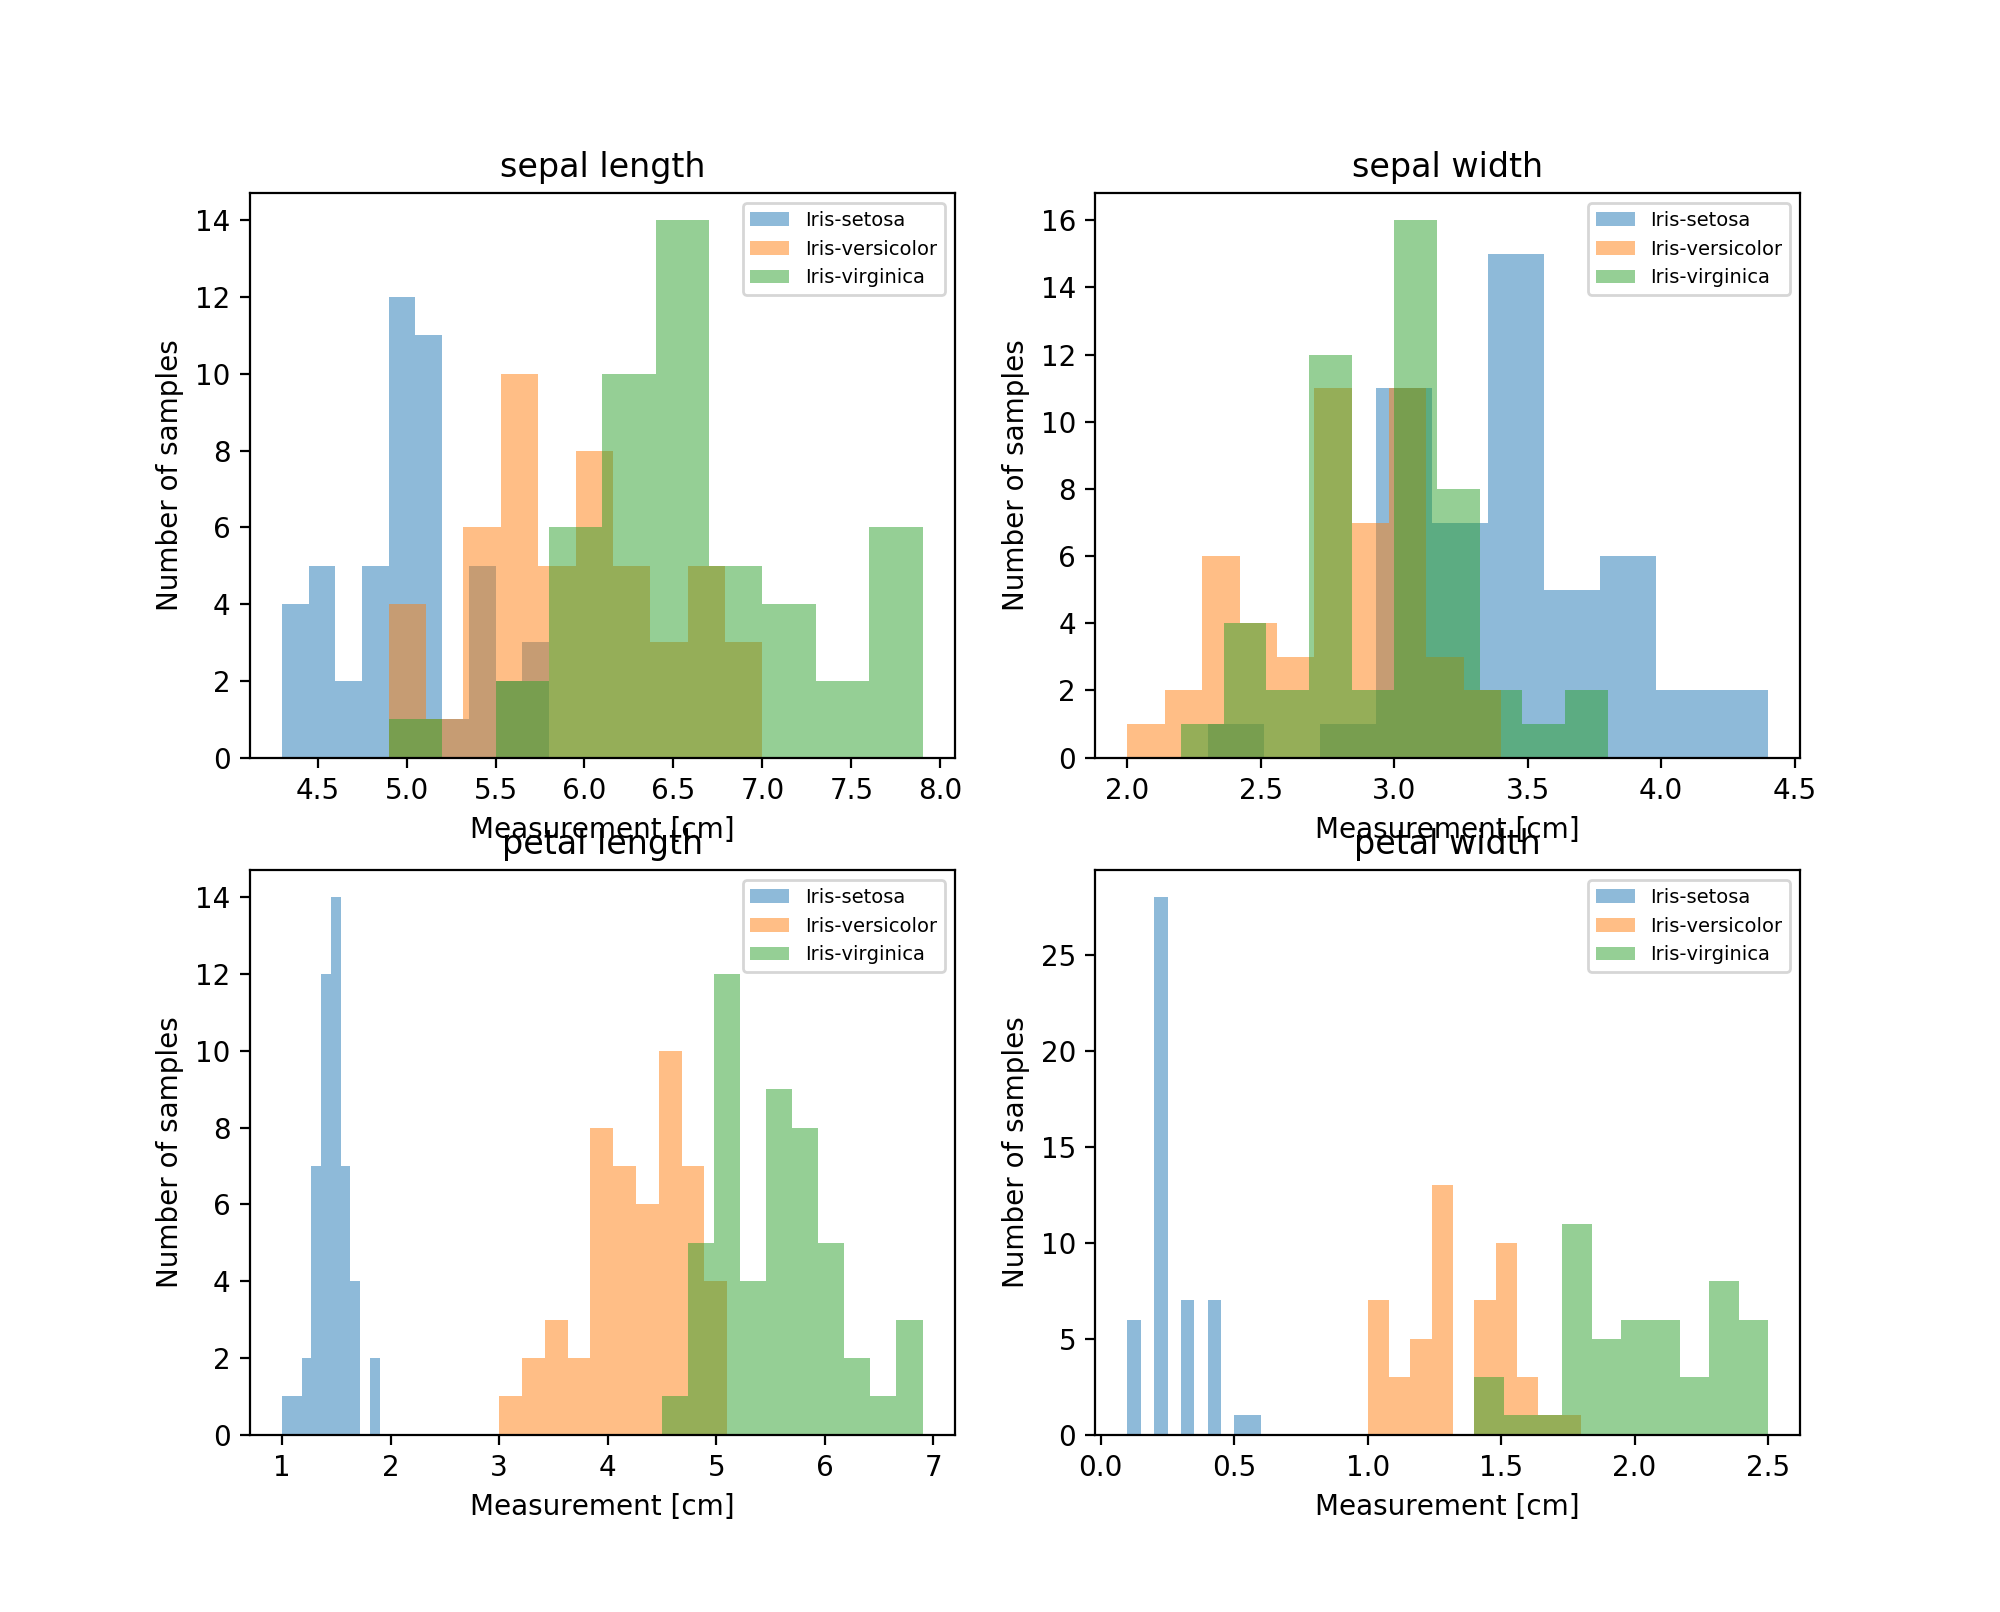
\includegraphics[width=\textwidth]{../images/iris_histograms.png}
    \caption{Histograms for each of the attributes of the Iris flowers.}
    \label{fig:histograms}
\end{figure}

Observe that for the petal widths and lengths, the features are almost linearly separable, e.g.
there is little overlap in the measurements from each of the classes for these features. In contrast,
the sepal lengths and widths have quite large overlaps. Since two of the features are almost
linearly separable, a linear classifier will be used in this project.

\section{Theory}

A linear classifier takes advantage of the fact that some classes may be separated by using a
linear operation on the dataset. Consider the scatter plot in \autoref{fig:petal_scatter_plot}.
Clearly, a line could be drawn in the middle of the void separating Iris Setosa samples from
Iris Versocolor samples. This line could then be used as a rule for classifying future samples
by just calculating which side of the line the new sample is on. It is not equally easy to
separate Versicolor from Virginica by using the same method - some of the Virginica samples overlap
with the Versicolor samples, and would then by misclassified. However, the error rate would be
quite small if the line is drawn in the middle of where the classes overlap. And in some case,
such an error rate would be considered acceptable.

In the case of the Iris dataset, there are four features to be considered. While a line in 2D
translates to a plane in 3D, it would become a hyperplane in datasets with a dimension N > 3.


The concept of separating

\begin{figure}
    \centering
    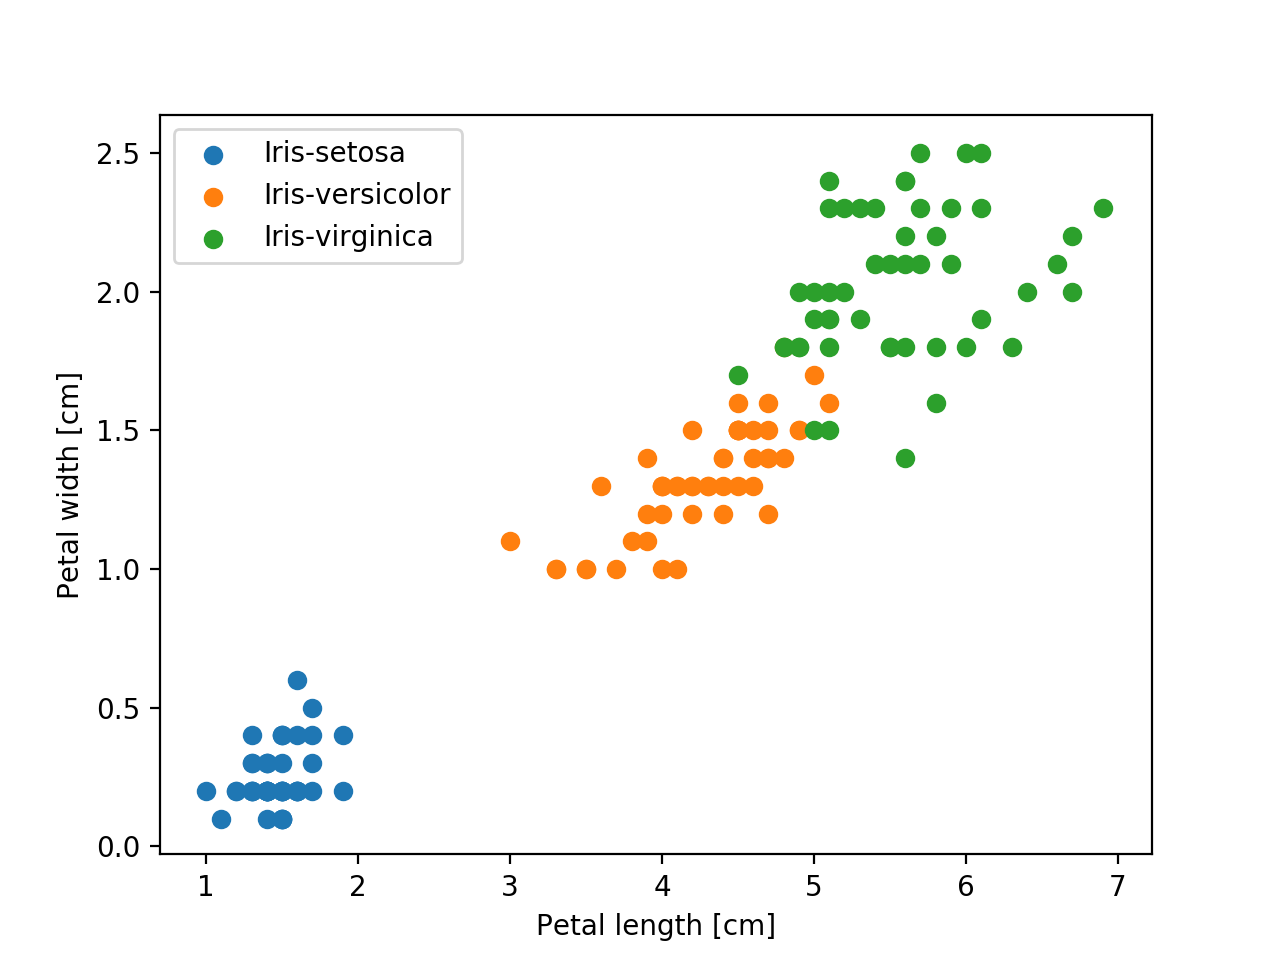
\includegraphics[width=\textwidth]{../images/petal_scatter.png}
    \caption{Histograms for each of the attributes of the Iris flowers.}
    \label{fig:petal_scatter_plot}
\end{figure}

\end{document}